\section{Image Analysis}

\subsection{Optical Music Recognition}

A lot of work has been done in the field of Optical Music Recognition or OMR - the process of converting written music notation so that it can be read by modern music notation software \ref{sec:ProfTools}.

Whilst the aim of this project is not OMR as much as scoring and analysing notation similarity, one of the techniques in particular is used for analysing manuscripts is common throughout most OMR applications and may have applications in this project.

It is noted in \citetitle{bainbridge2001challenge}\cite{bainbridge2001challenge} that:

\begin{quotation}
Before an OMR system can start recognising the shapes contained in an image, it must establish the size of the music notation being used. Staff lines are a reliable feature contained within a page, from which the staff height can be deduced, and consequently the size of the music notation. All reported OMR systems detect staff lines as the initial stage.
\end{quotation}

The technique essentially involves projecting the manuscript in the x-axis, collecting the pixels in either individual lines or buckets.

So, if the image is represented as a 1 bit (2 colour) image $P$ of width $x_{\text{max}}$ and height $y_{\text{max}}$, where $P_{xy}$denotes the value ($0$ or $1$) for a specific pixel at row $x$ column $y$, a summary count of pixels $C_0 C_1 ... C_{y_{\text{max}}}$ is generated for each row such that $C_i = \sum_{j = 0}^{x_\text{max} I(j, i)}$

\begin{figure}[h!]
  \centering
  \frame{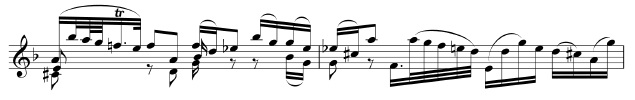
\includegraphics[width=\linewidth]{gfx/sonatas-partitas.jpg}}
  \caption{An excerpt from Bach's \emph{Sonatas Partitas}, obtained from http://www.virtualsheetmusic.com/score/SonatasPartitas.html}
  \label{fig:SonatasPartitas}
\end{figure}

\begin{figure}[h!]
  \centering
  \frame{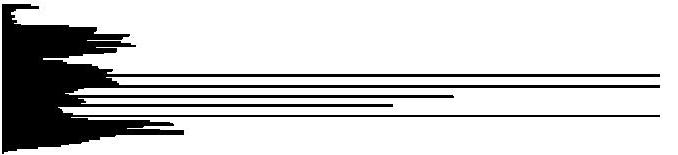
\includegraphics[width=\linewidth]{gfx/sonatas-partitas-projection.jpg}}
  \caption{The projection of the Sonatas Partitas piece extract in \ref{fig:SonatasPartitas}}
  \label{fig:SonatasPartitasProjection}
\end{figure}

An example section of score is shown in ~\ref{fig:SonatasPartitas} and it's resulting projection in ~\ref{fig:SonatasPartitasProjection}. You can clearly see the staff lines projecting far beyond the other noise of the piece.

We can now use this information to extract the notes from the staff lines via simple subtraction, to determine on which lines the notes are written, or even to determine orientation for further processing.

\subsection{Image Difference}

If you're handling simple 1 bit images, you can perform a simple image difference which just takes the first image, XOR'd with the second. The result (shown in Figure \ref{fig:CrochetDiff}) is a simple highlighting of the difference between the two.

\begin{figure}[h!]
  \centering
  \frame{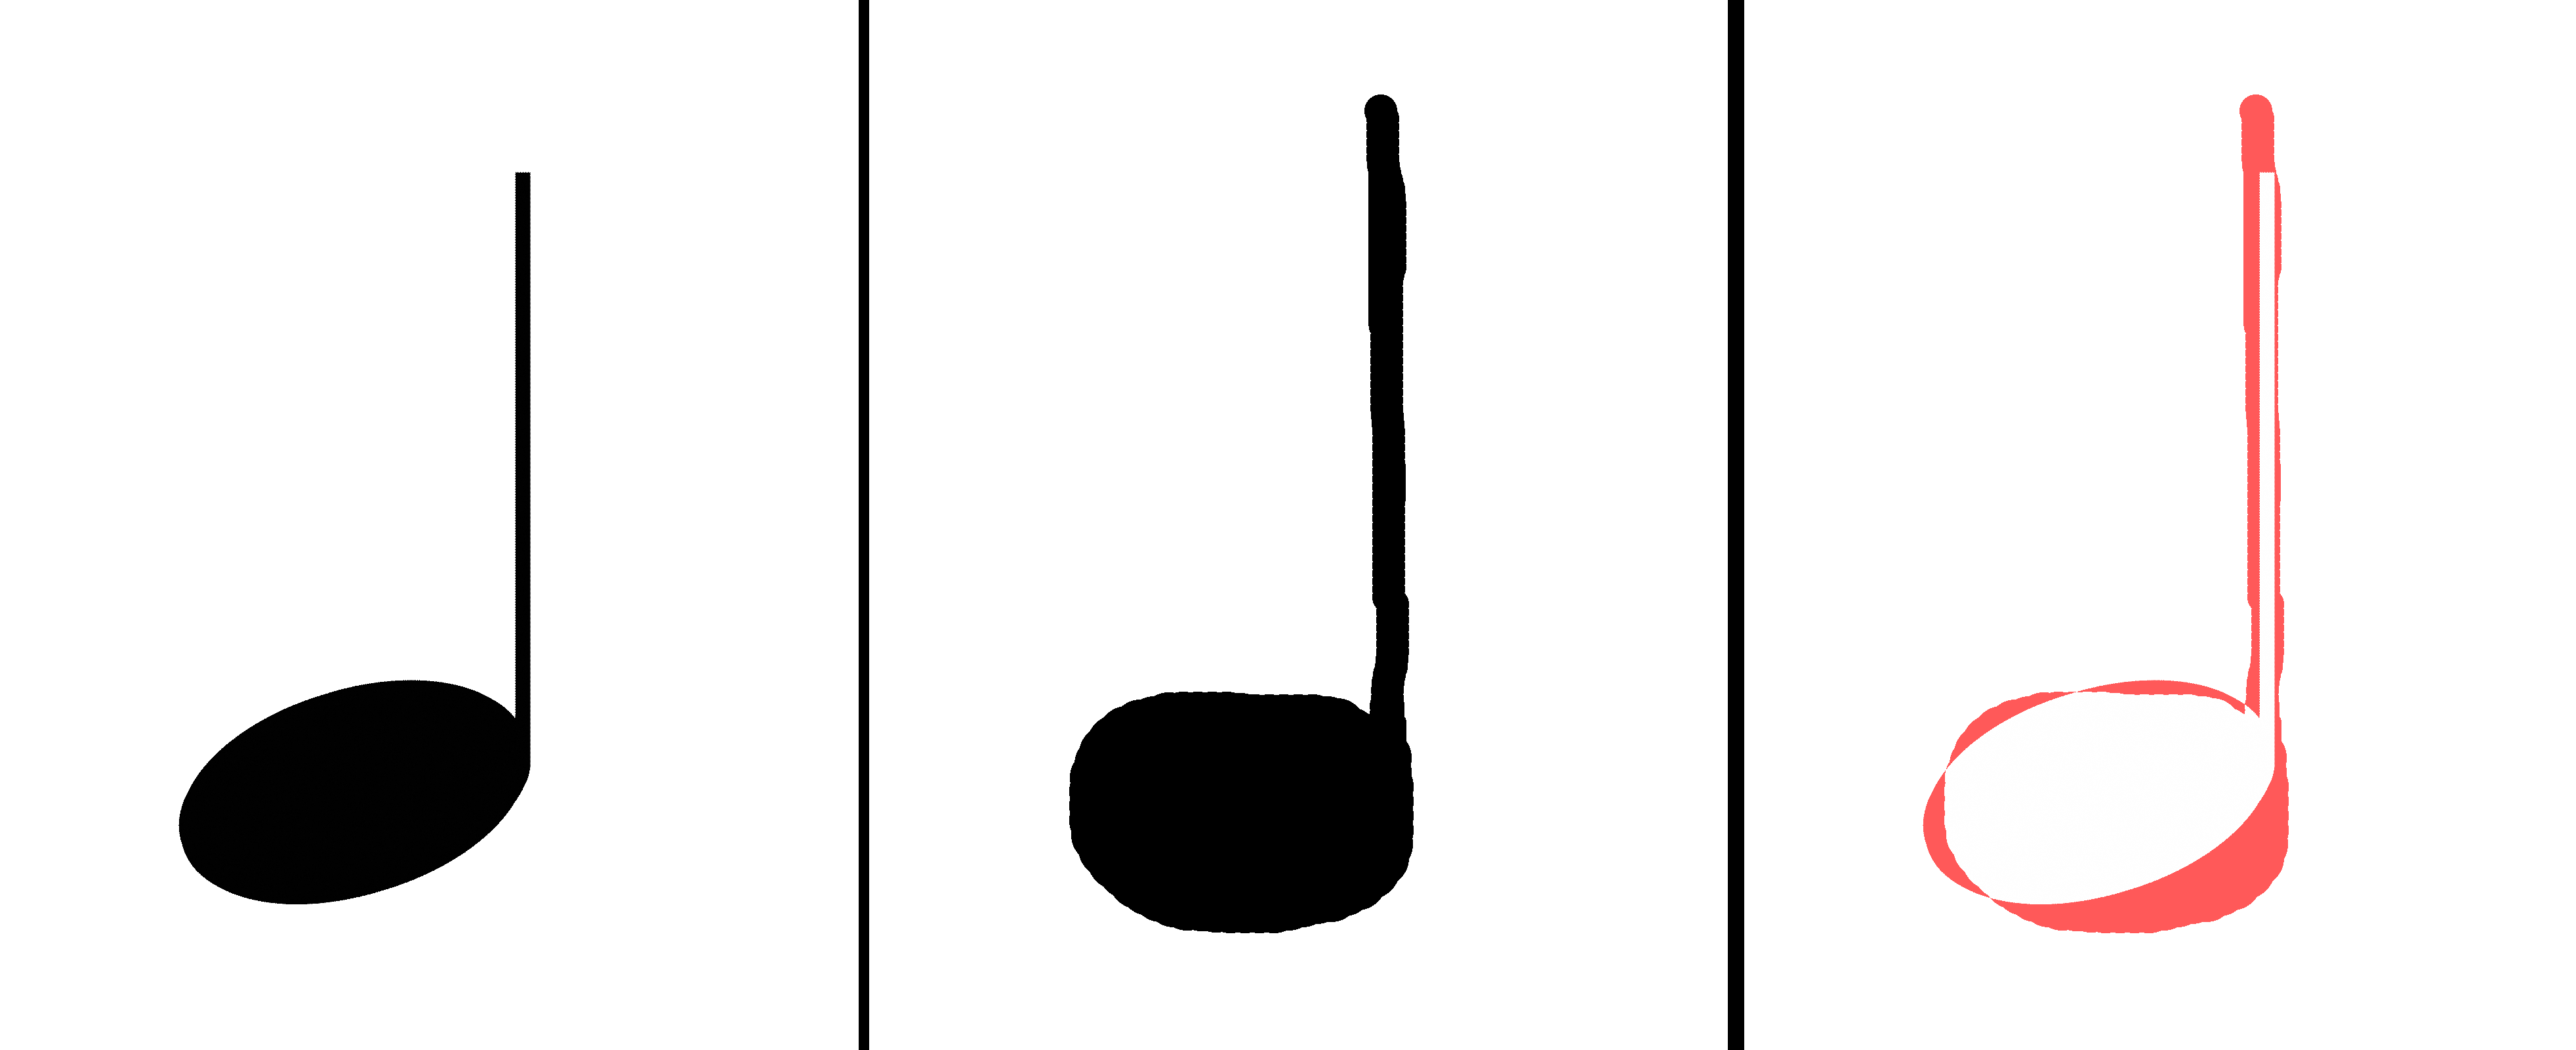
\includegraphics[width=\linewidth]{gfx/crochet-all.png}}
  \caption{Highlighting differences between a perfect and a hand-drawn crochet}
  \label{fig:CrochetDiff}
\end{figure}

A similar technique of image difference analysis can be applied to more complex images, however you often have to take into account the additional complexities of colour, compression-loss\footnote{} and normalisation of light levels. Indeed, when comparing two images using ImageMagick's\footnote{\url{http://www.imagemagick.org/}} compare function \footnote{\url{http://www.imagemagick.org/Usage/compare/\#compare}} although the defaults highlight changes quite clearly as in Figure \ref{fig:KittenDiff}, several metric options are offered\footnote{\url{http://www.imagemagick.org/Usage/compare/\#statistics}}.

\begin{figure}[h!]
  \centering
  \frame{
\includegraphics[width=\linewidth]{gfx/kitten-all.png}}
  \caption{Highlighting differences between two more complex images}
  \label{fig:KittenDiff}
\end{figure}


\subsection{Feature Matching}

Several techniques exist for feature matching such as SIFT\footnote{Scale Invariant Feature Transform - \url{http://en.wikipedia.org/wiki/Scale-invariant_feature_transform}} which allow you to identify key points on an image and then map them to another image containing the previous image inside it.

In an example I've investigated so far, I've discovered that it's more than possible to match musical notes in simple cases such as rotation (Figure \ref{fig:NoteRotate}) but further experiments have yet to be carried out regarding it's feasibility for this use case.


\begin{figure}[h!]
  \frame{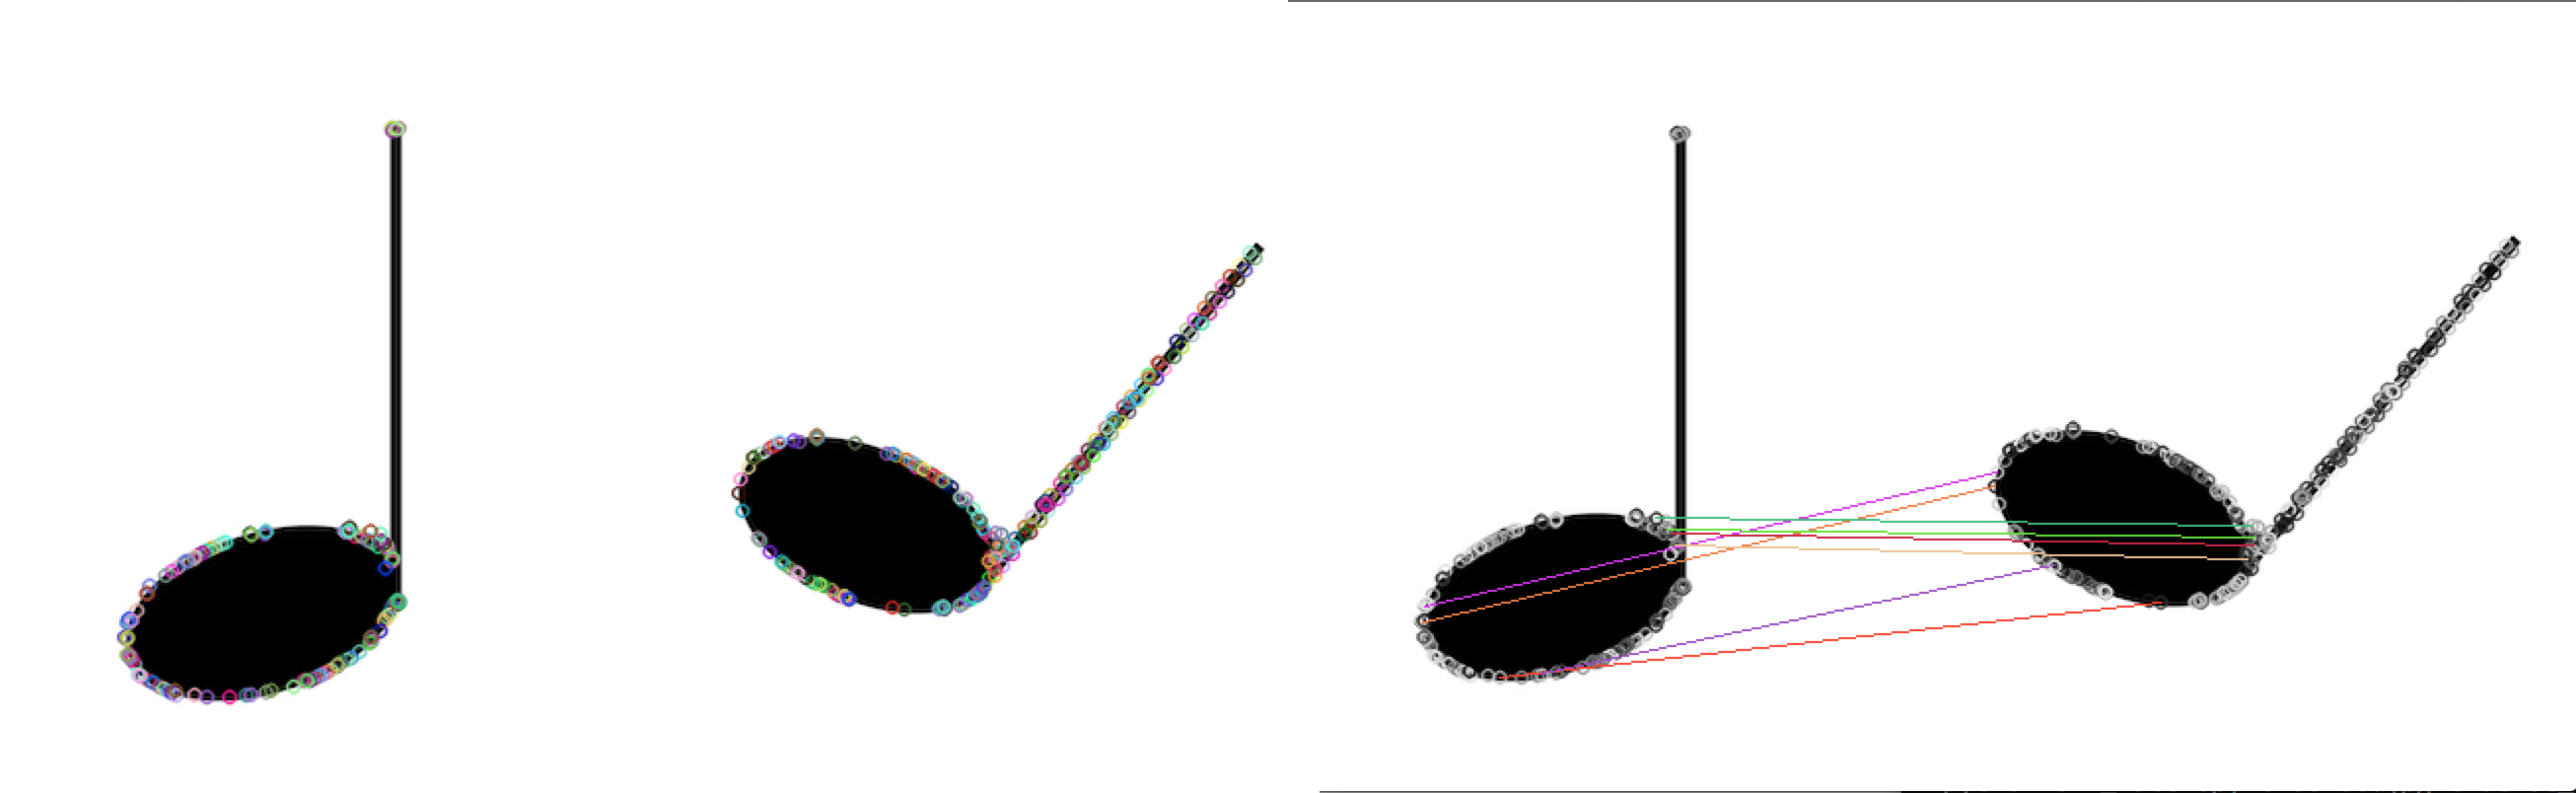
\includegraphics[width=0.6\linewidth]{gfx/feature-match.png}}
  \centering
  \caption{Example of feature matching notes using SIFT}
  \label{fig:NoteRotate}
\end{figure}

\subsection{Template Matching}

I've also attempted some examples of image segmentation using template matching, extracting components like the note head from the whole note as seen in Figure \ref{fig:templatematch}.

\begin{figure}[h!]
  \frame{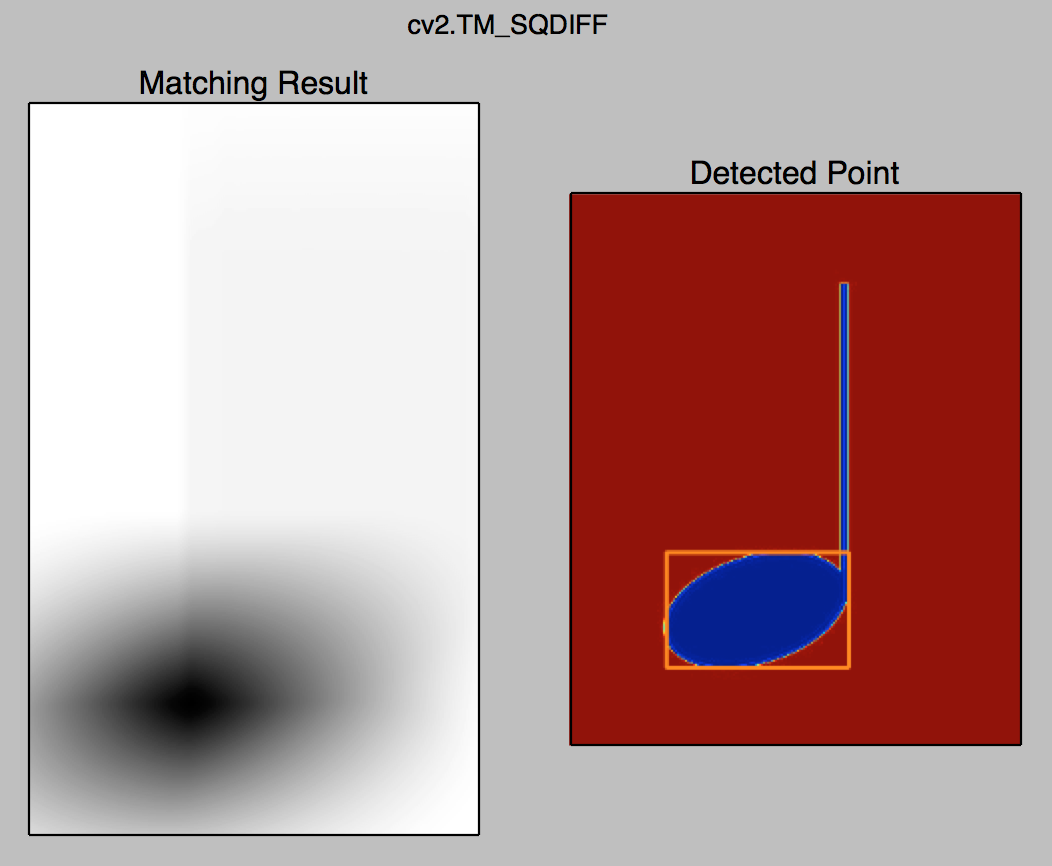
\includegraphics[width=0.6\linewidth]{gfx/template.png}}
  \centering
  \caption{Example of extracting note heads using template matching}
  \label{fig:templatematch}
\end{figure}

In this example, I've used the OpenCV library and utilised the SQ\_DIFF method (or sum of squared differences), to find similar image regions which is a popular method of producing a `matching' score.

This involves analysing each pixel in an image (or a region of an image) and comparing it to a reference pixel in a template. The score for two $n \times m$ images $x$ and $y$ is therefore generated using:

$$SSD_{xy} = \sum_{i = 0}^m \sum_{j = 0}^n (x(i, j) - y(i, j))^2$$

In the example I gave previously, we're only looking for a subsection or a partial template. We therefore if image $x$ is $m \times n$ and image $y$ is $a \times b$in size where $m \le a \land n \le b$, we can search each possible position $(k, l)$ for $y$ in $x$ with:

$$SSD_{xy}(k, l) = \sum_{i = 0}^m \sum_{j = 0}^n (x(i + k, j + l) - y(i, j))^2$$

and whichever positioning gives us the highest score is likely to be the best match.
